% This LaTeX document needs to be compiled with XeLaTeX.
\documentclass[10pt]{article}
\usepackage[utf8]{inputenc}
\usepackage{graphicx}
\usepackage[export]{adjustbox}
\graphicspath{ {./images/} }
\usepackage{amsmath}
\usepackage{amsfonts}
\usepackage{amssymb}
\usepackage[version=4]{mhchem}
\usepackage{stmaryrd}
\usepackage[fallback]{xeCJK}
\usepackage{polyglossia}
\usepackage{fontspec}
\setCJKmainfont{Noto Serif CJK KR}

\setmainlanguage{polish}
\setmainfont{CMU Serif}

\title{Egzamin maturalny }

\author{}
\date{}


\begin{document}
\maketitle
\begin{center}
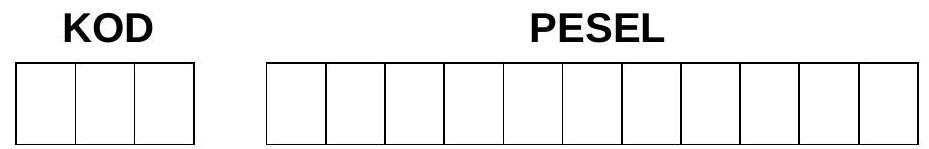
\includegraphics[max width=\textwidth]{2024_11_21_51cb67544fb9b029f01cg-01}
\end{center}

\section*{Miejsce na naklejkę.}
Sprawdź, czy kod na naklejce to M-100.

Jeżeli tak - przyklej naklejkę. Jeżeli nie - zgłoś to nauczycielowi.

\section*{Formuła 2023}
\section*{MATEMATYKA}
\section*{Poziom podstawowy}
Symbol arkusza\\
MMAP-P0-100-2305

\section*{DATA: 8 maja 2023 r. \\
 GoDzINA RozpoczECIA: 9:00 \\
 CZAS trWANIA: \(\mathbf{1 8 0}\) minut}
WYPEŁNIA ZESPÓŁ NADZORUJĄCY\\
Uprawnienia zdającego do:\\
dostosowania zasad oceniania dostosowania w zw. z dyskalkulią nieprzenoszenia zaznaczeń na kartę.

\section*{LICZBA PUNKTÓW DO UZYSKANIA: 46}
Przed rozpoczęciem pracy z arkuszem egzaminacyjnym

\begin{enumerate}
  \item Sprawdź, czy nauczyciel przekazał Ci właściwy arkusz egzaminacyjny, tj. arkusz we właściwej formule, z właściwego przedmiotu na właściwym poziomie.
  \item Jeżeli przekazano Ci niewłaściwy arkusz - natychmiast zgłoś to nauczycielowi. Nie rozrywaj banderol.
  \item Jeżeli przekazano Ci właściwy arkusz - rozerwij banderole po otrzymaniu takiego polecenia od nauczyciela. Zapoznaj się z instrukcją na stronie 2.\\

\includegraphics[max width=\textwidth, center]{2024_11_21_51cb67544fb9b029f01cg-02}
\end{enumerate}

\section*{Instrukcja dla zdającego}
\begin{enumerate}
  \item Sprawdź, czy arkusz egzaminacyjny zawiera 31 stron (zadania 1-31). Ewentualny brak zgłoś przewodniczącemu zespołu nadzorującego egzamin.
  \item Na pierwszej stronie arkusza oraz na karcie odpowiedzi wpisz swój numer PESEL i przyklej naklejkę z kodem.
  \item Symbol zamieszczony w nagłówku zadania oznacza, że rozwiązanie zadania zamkniętego musisz przenieść na kartę odpowiedzi.
  \item Odpowiedzi do zadań zamkniętych zaznacz na karcie odpowiedzi w części karty przeznaczonej dla zdającego. Zamaluj \(\square\) pola do tego przeznaczone. Błędne zaznaczenie otocz kółkiem ( i zaznacz właściwe.
  \item Pamiętaj, że pominięcie argumentacji lub istotnych obliczeń w rozwiązaniu zadania otwartego może spowodować, że za to rozwiązanie nie otrzymasz pełnej liczby punktów.
  \item Rozwiązania zadań i odpowiedzi wpisuj w miejscu na to przeznaczonym.
  \item Pisz czytelnie i używaj tylko długopisu lub pióra z czarnym tuszem lub atramentem.
  \item Nie używaj korektora, a błędne zapisy wyraźnie przekreśl.
  \item Nie wpisuj żadnych znaków w tabelkach przeznaczonych dla egzaminatora. Tabelki umieszczone są na marginesie przy odpowiednich zadaniach.
  \item Pamiętaj, że zapisy w brudnopisie nie będą oceniane.
  \item Możesz korzystać z Wybranych wzorów matematycznych, cyrkla i linijki oraz kalkulatora prostego. Upewnij się, czy przekazano Ci broszurę z okładką taką jak widoczna poniżej.\\

\includegraphics[max width=\textwidth, center]{2024_11_21_51cb67544fb9b029f01cg-02(1)}
\end{enumerate}

\section*{Zadania egzaminacyjne są wydrukowane na następnych stronach.}
Zadanie 1. (0-1) 마미\\
Na osi liczbowej zaznaczono sumę przedziałów.\\
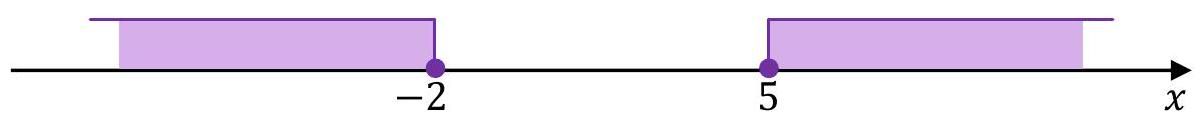
\includegraphics[max width=\textwidth, center]{2024_11_21_51cb67544fb9b029f01cg-04}

Dokończ zdanie. Wybierz właściwą odpowiedź spośród podanych.

Zbiór zaznaczony na osi jest zbiorem wszystkich rozwiązań nierówności\\
A. \(|x-3,5| \geq 1,5\)\\
B. \(|x-1,5| \geq 3,5\)\\
C. \(|x-3,5| \leq 1,5\)\\
D. \(|x-1,5| \leq 3,5\)\\

\includegraphics[max width=\textwidth, center]{2024_11_21_51cb67544fb9b029f01cg-04(2)}

\section*{Zadanie 2. (0-1) 마미}
Dokończ zdanie. Wybierz właściwą odpowiedź spośród podanych. Liczba \(\sqrt[3]{-\frac{27}{16}} \cdot \sqrt[3]{2}\) jest równa\\
A. \(\left(-\frac{3}{2}\right)\)\\
B. \(\frac{3}{2}\)\\
C. \(\frac{2}{3}\)\\
D. \(\left(-\frac{2}{3}\right)\)\\

\includegraphics[max width=\textwidth, center]{2024_11_21_51cb67544fb9b029f01cg-04(1)}

Zadanie 3. (0-2)\\
Wykaż, że dla każdej liczby naturalnej \(n \geq 1\) liczba \((2 n+1)^{2}-1\) jest podzielna przez 8.

\begin{center}
\begin{tabular}{|c|c|c|c|c|c|c|c|c|c|c|c|c|c|c|c|c|c|c|c|c|c|c|c|c|c|c|c|}
\hline
 &  &  &  &  &  &  &  &  &  &  &  &  &  &  &  &  &  &  &  &  &  &  &  &  &  &  &  \\
\hline
 &  &  &  &  &  &  &  &  &  &  &  &  &  &  &  &  &  &  &  &  &  &  &  &  &  &  &  \\
\hline
 &  &  &  &  &  &  &  &  &  &  &  &  &  &  &  &  &  &  &  &  &  &  &  &  &  &  &  \\
\hline
 &  &  &  &  &  &  &  &  &  &  &  &  &  &  &  &  &  &  &  &  &  &  &  &  &  &  &  \\
\hline
 &  &  &  &  &  &  &  &  &  &  &  &  &  &  &  &  &  &  &  &  &  &  &  &  &  &  &  \\
\hline
 &  &  &  &  &  &  &  &  &  &  &  &  &  &  &  &  &  &  &  &  &  &  &  &  &  &  &  \\
\hline
 &  &  &  &  &  &  &  &  &  &  &  &  &  &  &  &  &  &  &  &  &  &  &  &  &  &  &  \\
\hline
 &  &  &  &  &  &  &  &  &  &  &  &  &  &  &  &  &  &  &  &  &  &  &  &  &  &  &  \\
\hline
 &  &  &  &  &  &  &  &  &  &  &  &  &  &  &  &  &  &  &  &  &  &  &  &  &  &  &  \\
\hline
 &  &  &  &  &  &  &  &  &  &  &  &  &  &  &  &  &  &  &  &  &  &  &  &  &  &  &  \\
\hline
 &  &  &  &  &  &  &  &  &  &  &  &  &  &  &  &  &  &  &  &  &  &  &  &  &  &  &  \\
\hline
 &  &  &  &  &  &  &  &  &  &  &  &  &  &  &  &  &  &  &  &  &  &  &  &  &  &  &  \\
\hline
 &  &  &  &  &  &  &  &  &  &  &  &  &  &  &  &  &  &  &  &  &  &  &  &  &  &  &  \\
\hline
 &  &  &  &  &  &  &  &  &  &  &  &  &  &  &  &  &  &  &  &  &  &  &  &  &  &  &  \\
\hline
 &  &  &  &  &  &  &  &  &  &  &  &  &  &  &  &  &  &  &  &  &  &  &  &  &  &  &  \\
\hline
 &  &  &  &  &  &  &  &  &  &  &  &  &  &  &  &  &  &  &  &  &  &  &  &  &  &  &  \\
\hline
 &  &  &  &  &  &  &  &  &  &  &  &  &  &  &  &  &  &  &  &  &  &  &  &  &  &  &  \\
\hline
 &  &  &  &  &  &  &  &  &  &  &  &  &  &  &  &  &  &  &  &  &  &  &  &  &  &  &  \\
\hline
 &  &  &  &  &  &  &  &  &  &  &  &  &  &  &  &  &  &  &  &  &  &  &  &  &  &  &  \\
\hline
 &  &  &  &  &  &  &  &  &  &  &  &  &  &  &  &  &  &  &  &  &  &  &  &  &  &  &  \\
\hline
 &  &  &  &  &  &  &  &  &  &  &  &  &  &  &  &  &  &  &  &  &  &  &  &  &  &  &  \\
\hline
 &  &  &  &  &  &  &  &  &  &  &  &  &  &  &  &  &  &  &  &  &  &  &  &  &  &  &  \\
\hline
 &  &  &  &  &  &  &  &  &  &  &  &  &  &  &  &  &  &  &  &  &  &  &  &  &  &  &  \\
\hline
 &  &  &  &  &  &  &  &  &  &  &  &  &  &  &  &  &  &  &  &  &  &  &  &  &  &  &  \\
\hline

\includegraphics[max width=\textwidth]{2024_11_21_51cb67544fb9b029f01cg-05(1)}
 &  &  &  &  &  &  &  &  &  &  &  &  &  &  &  &  &  &  &  &  &  &  &  &  &  &  &  \\
\hline
 &  &  &  &  &  &  &  &  &  &  &  &  &  &  &  &  &  &  &  &  &  &  &  &  &  &  &  \\
\hline

\includegraphics[max width=\textwidth]{2024_11_21_51cb67544fb9b029f01cg-05}
 &  &  &  &  &  &  &  &  &  &  &  &  &  &  &  &  &  &  &  &  &  &  &  &  &  &  &  \\
\hline
 &  &  &  &  &  &  &  &  &  &  &  &  &  &  &  &  &  &  &  &  &  &  &  &  &  &  &  \\
\hline
 &  &  &  &  &  &  &  &  &  &  &  &  &  &  &  &  &  &  &  &  &  &  &  &  &  &  &  \\
\hline
 &  &  &  &  &  &  &  &  &  &  &  &  &  &  &  &  &  &  &  &  &  &  &  &  &  &  &  \\
\hline
 &  &  &  &  &  &  &  &  &  &  &  &  &  &  &  &  &  &  &  &  &  &  &  &  &  &  &  \\
\hline
 &  &  &  &  &  &  &  &  &  &  &  &  &  &  &  &  &  &  &  &  &  &  &  &  &  &  &  \\
\hline
 &  &  &  &  &  &  &  &  &  &  &  &  &  &  &  &  &  &  &  &  &  &  &  &  &  &  &  \\
\hline
 &  &  &  &  &  &  &  &  &  &  &  &  &  &  &  &  &  &  &  &  &  &  &  &  &  &  &  \\
\hline
 &  &  &  &  &  &  &  &  &  &  &  &  &  &  &  &  &  &  &  &  &  &  &  &  &  &  &  \\
\hline
. &  &  &  &  &  &  &  &  &  &  &  &  &  &  &  &  &  &  &  &  &  &  &  &  &  &  &  \\
\hline
 &  &  &  &  &  &  &  &  &  &  &  &  &  &  &  &  &  &  &  &  &  &  &  &  &  &  &  \\
\hline
 &  &  &  &  &  &  &  &  &  &  &  &  &  &  &  &  &  &  &  &  &  &  &  &  &  &  &  \\
\hline
 &  &  &  &  &  &  &  &  &  &  &  &  &  &  &  &  &  &  &  &  &  &  &  &  &  &  &  \\
\hline
 &  &  &  &  &  &  &  &  &  &  &  &  &  &  &  &  &  &  &  &  &  &  &  &  &  &  &  \\
\hline
- &  &  &  &  &  &  &  &  &  &  &  &  &  &  &  &  &  &  &  &  &  &  &  &  &  &  &  \\
\hline
 &  &  &  &  &  &  &  &  &  &  &  &  &  &  &  &  &  &  &  &  &  &  &  &  &  &  &  \\
\hline
 &  &  &  &  &  &  &  &  &  &  &  &  &  &  &  &  &  &  &  &  &  &  &  &  &  &  &  \\
\hline
 &  &  &  &  &  &  &  &  &  &  &  &  &  &  &  &  &  &  &  &  &  &  &  &  &  &  &  \\
\hline
 &  &  &  &  &  &  &  &  &  &  &  &  &  &  &  &  &  &  &  &  &  &  &  &  &  &  &  \\
\hline
\end{tabular}
\end{center}

Zadanie 4. (0-1) 무이\\
Dokończ zdanie. Wybierz właściwą odpowiedź spośród podanych.\\
Liczba \(\log _{9} 27+\log _{9} 3\) jest równa\\
A. 81\\
B. 9\\
C. 4\\
D. 2

\begin{center}
\begin{tabular}{|c|c|c|c|c|c|c|c|c|c|c|c|c|c|c|c|c|c|c|c|c|c|c|c|}
\hline
 & Brudn & opis &  &  &  &  &  &  &  &  &  &  &  &  &  &  &  &  &  &  &  &  &  \\
\hline
 &  &  &  &  &  &  &  &  &  &  &  &  &  &  &  &  &  &  &  &  &  &  &  \\
\hline
 &  &  &  &  &  &  &  &  &  &  &  &  &  &  &  &  &  &  &  &  &  &  &  \\
\hline
 &  &  &  &  &  &  &  &  &  &  &  &  &  &  &  &  &  &  &  &  &  &  &  \\
\hline
 &  &  &  &  &  &  &  &  &  &  &  &  &  &  &  &  &  &  &  &  &  &  &  \\
\hline
 &  &  &  &  &  &  &  &  &  &  &  &  &  &  &  &  &  &  &  &  &  &  &  \\
\hline
 &  &  &  &  &  &  &  &  &  &  &  &  &  &  &  &  &  &  &  &  &  &  &  \\
\hline
 &  &  &  &  &  &  &  &  &  &  &  &  &  &  &  &  &  &  &  &  &  &  &  \\
\hline
 &  &  &  &  &  &  &  &  &  &  &  &  &  &  &  &  &  &  &  &  &  &  &  \\
\hline
 &  &  &  &  &  &  &  &  &  &  &  &  &  &  &  &  &  &  &  &  &  &  &  \\
\hline
 &  &  &  &  &  &  &  &  &  &  &  &  &  &  &  &  &  &  &  &  &  &  &  \\
\hline
 &  &  &  &  &  &  &  &  &  &  &  &  &  &  &  &  &  &  &  &  &  &  &  \\
\hline
 &  &  &  &  &  &  &  &  &  &  &  &  &  &  &  &  &  &  &  &  &  &  &  \\
\hline
 &  &  &  &  &  &  &  &  &  &  &  &  &  &  &  &  &  &  &  &  &  &  &  \\
\hline
\end{tabular}
\end{center}

\section*{Zadanie 5. (0-1) 다미}
Dokończ zdanie. Wybierz właściwą odpowiedź spośród podanych.\\
Dla każdej liczby rzeczywistej \(a\) wyrażenie \((2 a-3)^{2}-(2 a+3)^{2}\) jest równe\\
A. \(-24 a\)\\
B. 0\\
C. 18\\
D. \(16 a^{2}-24 a\)

\begin{center}
\begin{tabular}{|c|c|c|c|c|c|c|c|c|c|c|c|c|c|c|c|c|c|c|c|c|c|c|}
\hline
\multicolumn{4}{|l|}{Brudnopis} &  &  &  &  &  &  &  &  &  &  &  &  &  &  &  &  &  &  &  \\
\hline
 &  &  &  &  &  &  &  &  &  &  &  &  &  &  &  &  &  &  &  &  &  &  \\
\hline
 &  &  &  &  &  &  &  &  &  &  &  &  &  &  &  &  &  &  &  &  &  &  \\
\hline
 &  &  &  &  &  &  &  &  &  &  &  &  &  &  &  &  &  &  &  &  &  &  \\
\hline
 &  &  &  &  &  &  &  &  &  &  &  &  &  &  &  &  &  &  &  &  &  &  \\
\hline
 &  &  &  &  &  &  &  &  &  &  &  &  &  &  &  &  &  &  &  &  &  &  \\
\hline
 &  &  &  &  &  &  &  &  &  &  &  &  &  &  &  &  &  &  &  &  &  &  \\
\hline
 &  &  &  &  &  &  &  &  &  &  &  &  &  &  &  &  &  &  &  &  &  &  \\
\hline
 &  &  &  &  &  &  &  &  &  &  &  &  &  &  &  &  &  &  &  &  &  &  \\
\hline
 &  &  &  &  &  &  &  &  &  &  &  &  &  &  &  &  &  &  &  &  &  &  \\
\hline
 &  &  &  &  &  &  &  &  &  &  &  &  &  &  &  &  &  &  &  &  &  &  \\
\hline
 &  &  &  &  &  &  &  &  &  &  &  &  &  &  &  &  &  &  &  &  &  &  \\
\hline
 &  &  &  &  &  &  &  &  &  &  &  &  &  &  &  &  &  &  &  &  &  &  \\
\hline
 &  &  &  &  &  &  &  &  &  &  &  &  &  &  &  &  &  &  &  &  &  &  \\
\hline
 &  &  &  &  &  &  &  &  &  &  &  &  &  &  &  &  &  &  &  &  &  &  \\
\hline
 &  &  &  &  &  &  &  &  &  &  &  &  &  &  &  &  &  &  &  &  &  &  \\
\hline
 &  &  &  &  &  &  &  &  &  &  &  &  &  &  &  &  &  &  &  &  &  &  \\
\hline
 &  &  &  &  &  &  &  &  &  &  &  &  &  &  &  &  &  &  &  &  &  &  \\
\hline
\end{tabular}
\end{center}

Zadanie 6. (0-1) 무이\\
Dokończ zdanie. Wybierz właściwą odpowiedź spośród podanych.\\
Zbiorem wszystkich rozwiązań nierówności

\[
-2(x+3) \leq \frac{2-x}{3}
\]

jest przedział\\
A. \((-\infty,-4]\)\\
B. \((-\infty, 4]\)\\
C. \([-4, \infty)\)\\
D. \([4, \infty)\)

\begin{center}
\begin{tabular}{|c|c|c|c|c|c|c|c|c|c|c|c|c|c|c|c|c|c|c|c|c|}
\hline
 & Brudnop & opis &  &  &  &  &  &  &  &  & - &  &  & . & - & - &  &  &  &  \\
\hline
 &  &  &  &  &  &  &  &  &  &  &  &  &  &  &  &  &  &  &  &  \\
\hline
 &  &  &  &  &  &  &  &  &  &  &  &  &  &  &  &  &  &  &  &  \\
\hline
 &  &  &  &  &  &  &  &  &  &  &  &  &  &  &  &  &  &  &  &  \\
\hline
 &  &  &  &  &  &  &  &  &  &  &  &  &  &  &  &  &  &  &  &  \\
\hline
 &  &  &  &  &  &  &  &  &  &  &  &  &  &  &  &  &  &  &  &  \\
\hline
 &  &  &  &  &  &  &  &  &  &  &  &  &  &  &  &  &  &  &  &  \\
\hline
 &  &  &  &  &  &  &  &  &  &  &  &  &  &  &  &  &  &  &  &  \\
\hline
 &  &  &  &  &  &  &  &  &  &  &  &  &  &  &  &  &  &  &  &  \\
\hline
 &  &  &  &  &  &  &  &  &  &  &  &  &  &  &  &  &  &  &  &  \\
\hline
 &  &  &  &  &  &  &  &  &  &  &  &  &  &  &  &  &  &  &  &  \\
\hline
 &  &  &  &  &  &  &  &  &  &  &  &  &  &  &  &  &  &  &  &  \\
\hline
 &  &  &  &  &  &  &  &  &  &  &  &  &  &  &  &  &  &  &  &  \\
\hline
 &  &  &  &  &  &  &  &  &  &  &  &  &  &  &  &  &  &  &  &  \\
\hline
 &  &  &  &  &  &  &  &  &  &  &  &  &  &  &  &  &  &  &  &  \\
\hline
\end{tabular}
\end{center}

\section*{Zadanie 7. (0-1)}
Dokończ zdanie. Wybierz właściwą odpowiedź spośród podanych. Jednym z rozwiązań równania \(\sqrt{3}\left(x^{2}-2\right)(x+3)=0\) jest liczba\\
A. 3\\
B. 2\\
C. \(\sqrt{3}\)\\
D. \(\sqrt{2}\)\\

\includegraphics[max width=\textwidth, center]{2024_11_21_51cb67544fb9b029f01cg-07}

Zadanie 8. (0-1) 마미\\
Dokończ zdanie. Wybierz właściwą odpowiedź spośród podanych.

Równanie \(\frac{(x+1)(x-1)^{2}}{(x-1)(x+1)^{2}}=0\) w zbiorze liczb rzeczywistych\\
A. nie ma rozwiązania.\\
B. ma dokładnie jedno rozwiązanie: -1 .\\
C. ma dokładnie jedno rozwiązanie: 1 .\\
D. ma dokładnie dwa rozwiązania: -1 oraz 1 .

\begin{center}
\begin{tabular}{|c|c|c|c|c|c|c|c|c|c|c|c|c|c|c|c|c|c|c|c|c|c|c|c|c|c|c|}
\hline
\multicolumn{5}{|l|}{Brudnopis} &  &  &  &  &  &  &  &  &  &  &  &  &  &  &  &  &  &  &  &  &  &  \\
\hline
 &  &  &  &  &  &  &  &  &  &  &  &  &  &  &  &  &  &  &  &  &  &  &  &  &  &  \\
\hline
 &  &  &  &  &  &  &  &  &  &  &  &  &  &  &  &  &  &  &  &  &  &  &  &  &  &  \\
\hline
 &  &  &  &  &  &  &  &  &  &  &  &  &  &  &  &  &  &  &  &  &  &  &  &  &  &  \\
\hline
 &  &  &  &  &  &  &  &  &  &  &  &  &  &  &  &  &  &  &  &  &  &  &  &  &  &  \\
\hline
 &  &  &  &  &  &  &  &  &  &  &  &  &  &  &  &  &  &  &  &  &  &  &  &  &  &  \\
\hline
 &  &  &  &  &  &  &  &  &  &  &  &  &  &  &  &  &  &  &  &  &  &  &  &  &  &  \\
\hline
 &  &  &  &  &  &  &  &  &  &  &  &  &  &  &  &  &  &  &  &  &  &  &  &  &  &  \\
\hline
 &  &  &  &  &  &  &  &  &  &  &  &  &  &  &  &  &  &  &  &  &  &  &  &  &  &  \\
\hline
 &  &  &  &  &  &  &  &  &  &  &  &  &  &  &  &  &  &  &  &  &  &  &  &  &  &  \\
\hline
 &  &  &  &  &  &  &  &  &  &  &  &  &  &  &  &  &  &  &  &  &  &  &  &  &  &  \\
\hline
 &  &  &  &  &  &  &  &  &  &  &  &  &  &  &  &  &  &  &  &  &  &  &  &  &  &  \\
\hline
\end{tabular}
\end{center}

Zadanie 9. (0-3)\\
Rozwiąż równanie

\[
3 x^{3}-2 x^{2}-12 x+8=0
\]

Zapisz obliczenia.\\

\includegraphics[max width=\textwidth, center]{2024_11_21_51cb67544fb9b029f01cg-08}\\

\includegraphics[max width=\textwidth, center]{2024_11_21_51cb67544fb9b029f01cg-09}

Zadanie 10. (0-1) 마미\\
Na rysunku przedstawiono interpretację geometryczną w kartezjańskim układzie współrzędnych \((x, y)\) jednego z niżej zapisanych układów równań A-D.\\
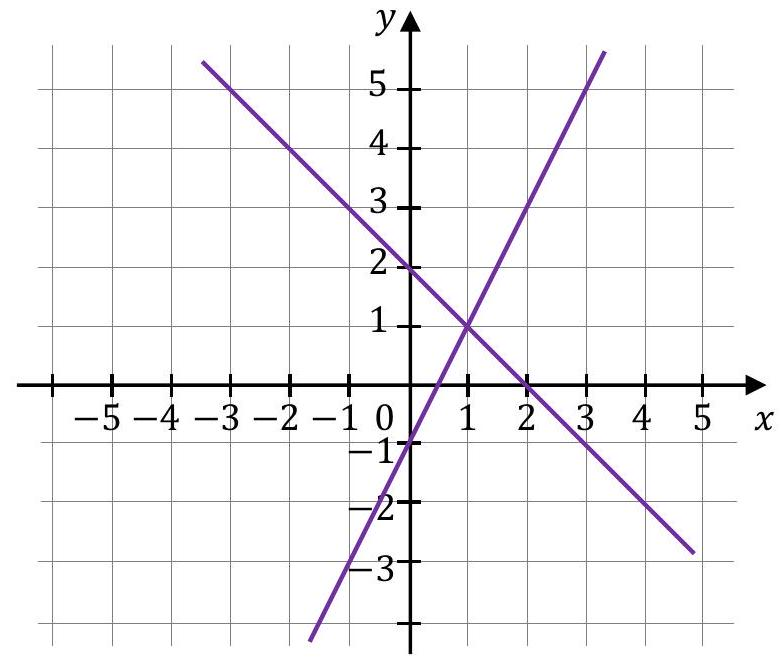
\includegraphics[max width=\textwidth, center]{2024_11_21_51cb67544fb9b029f01cg-10}

Dokończ zdanie. Wybierz właściwą odpowiedź spośród podanych.

Układem równań, którego interpretację geometryczną przedstawiono na rysunku, jest\\
A. \(\left\{\begin{array}{l}y=-x+2 \\ y=-2 x+1\end{array}\right.\)\\
B. \(\left\{\begin{array}{l}y=x-2 \\ y=-2 x-1\end{array}\right.\)\\
C. \(\left\{\begin{array}{l}y=x-2 \\ y=2 x+1\end{array}\right.\)\\
D. \(\left\{\begin{array}{l}y=-x+2 \\ y=2 x-1\end{array}\right.\)\\

\includegraphics[max width=\textwidth, center]{2024_11_21_51cb67544fb9b029f01cg-10(1)}

Zadanie 11. (0-2)\\
Dany jest prostokąt o bokach długości \(a\) i \(b\), gdzie \(a>b\). Obwód tego prostokąta jest równy 30. Jeden z boków prostokąta jest o 5 krótszy od drugiego.

Uzupełnij zdanie. Wybierz dwie właściwe odpowiedzi spośród oznaczonych literami A-F i wpisz te litery w wykropkowanych miejscach.

Zależności między długościami boków tego prostokąta zapisano w układach równań oznaczonych literami: \(\qquad\) oraz \(\qquad\) .\\
A. \(\left\{\begin{array}{l}2 a b=30 \\ a-b=5\end{array}\right.\)\\
B. \(\left\{\begin{array}{l}2 a+b=30 \\ a=5 b\end{array}\right.\)\\
C. \(\left\{\begin{array}{l}2(a+b)=30 \\ b=a-5\end{array}\right.\)\\
D. \(\left\{\begin{array}{l}2 a+2 b=30 \\ b=5 a\end{array}\right.\)\\
E. \(\left\{\begin{array}{l}2 a+2 b=30 \\ a-b=5\end{array}\right.\)\\
F. \(\left\{\begin{array}{l}a+b=30 \\ a=b+5\end{array}\right.\)\\

\includegraphics[max width=\textwidth, center]{2024_11_21_51cb67544fb9b029f01cg-11}

\section*{Zadanie 12.}
W kartezjańskim układzie współrzędnych \((x, y)\) narysowano wykres funkcji \(y=f(x)\) (zobacz rysunek).\\
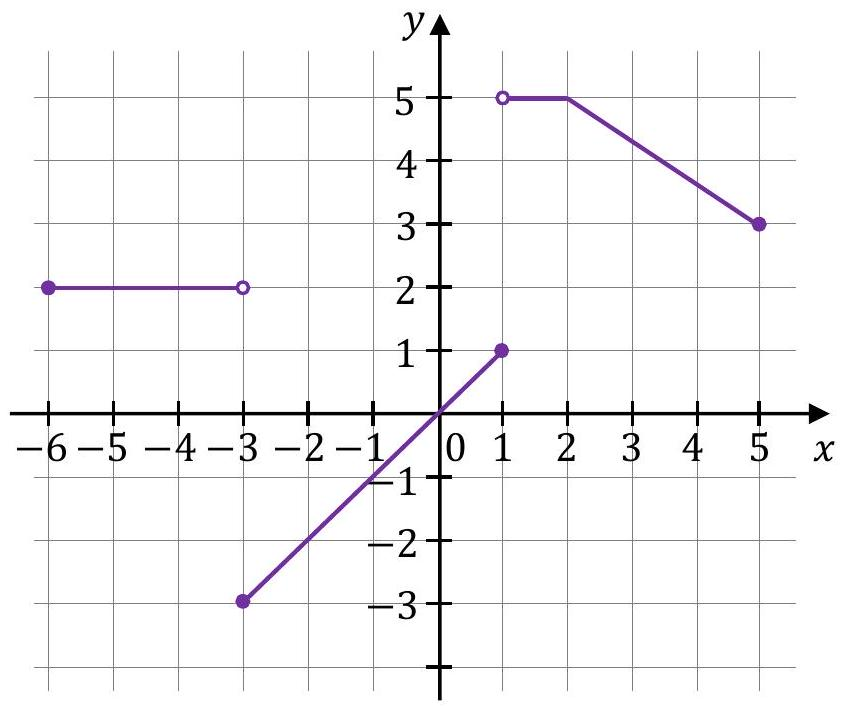
\includegraphics[max width=\textwidth, center]{2024_11_21_51cb67544fb9b029f01cg-12(2)}

\section*{Zadanie 12.1. (0-1)}
Dokończ zdanie. Wybierz właściwą odpowiedź spośród podanych.\\
Dziedziną funkcji \(f\) jest zbiór\\
A. \([-6,5]\)\\
B. \((-6,5)\)\\
C. \((-3,5]\)\\
D. \([-3,5]\)\\

\includegraphics[max width=\textwidth, center]{2024_11_21_51cb67544fb9b029f01cg-12(1)}

\section*{Zadanie 12.2. (0-1) 四}
Dokończ zdanie. Wybierz właściwą odpowiedź spośród podanych.\\
Największa wartość funkcji \(f\) w przedziale \([-4,1]\) jest równa\\
A. 0\\
B. 1\\
C. 2\\
D. 5\\

\includegraphics[max width=\textwidth, center]{2024_11_21_51cb67544fb9b029f01cg-12}

Zadanie 12.3. (0-1)\\
Dokończ zdanie. Wybierz właściwą odpowiedź spośród podanych.\\
Funkcja \(f\) jest malejąca w zbiorze\\
A. \([-6,-3)\)\\
B. \([-3,1]\)\\
C. \((1,2]\)\\
D. \([2,5]\)

\begin{center}
\begin{tabular}{|c|c|c|c|c|c|c|c|c|c|c|c|c|c|c|c|c|c|c|c|c|c|c|c|c|c|c|c|c|c|c|}
\hline
\multicolumn{5}{|l|}{Brudnopis} &  &  &  &  &  &  &  &  &  &  &  &  &  &  &  &  &  &  &  &  &  &  &  &  &  &  \\
\hline
 &  &  &  &  &  &  &  &  &  &  &  &  &  &  &  &  &  &  &  &  &  &  &  &  &  &  &  &  &  &  \\
\hline
 &  &  &  &  &  &  &  &  &  &  &  &  &  &  &  &  &  &  &  &  &  &  &  &  &  &  &  &  &  &  \\
\hline
 &  &  &  &  &  &  &  &  &  &  &  &  &  &  &  &  &  &  &  &  &  &  &  &  &  &  &  &  &  &  \\
\hline
 &  &  &  &  &  &  &  &  &  &  &  &  &  &  &  &  &  &  &  &  &  &  &  &  &  &  &  &  &  &  \\
\hline
 &  &  &  &  &  &  &  &  &  &  &  &  &  &  &  &  &  &  &  &  &  &  &  &  &  &  &  &  &  &  \\
\hline
 &  &  &  &  &  &  &  &  &  &  &  &  &  &  &  &  &  &  &  &  &  &  &  &  &  &  &  &  &  &  \\
\hline
 &  &  &  &  &  &  &  &  &  &  &  &  &  &  &  &  &  &  &  &  &  &  &  &  &  &  &  &  &  &  \\
\hline
 &  &  &  &  &  &  &  &  &  &  &  &  &  &  &  &  &  &  &  &  &  &  &  &  &  &  &  &  &  &  \\
\hline
\end{tabular}
\end{center}

\section*{Zadanie 13. (0-1) 무미}
Funkcja liniowa \(f\) jest określona wzorem \(f(x)=a x+b\), gdzie \(a\) i \(b\) są pewnymi liczbami rzeczywistymi. Na rysunku obok przedstawiono fragment wykresu funkcji \(f\) w kartezjańskim układzie współrzędnych \((x, y)\).\\
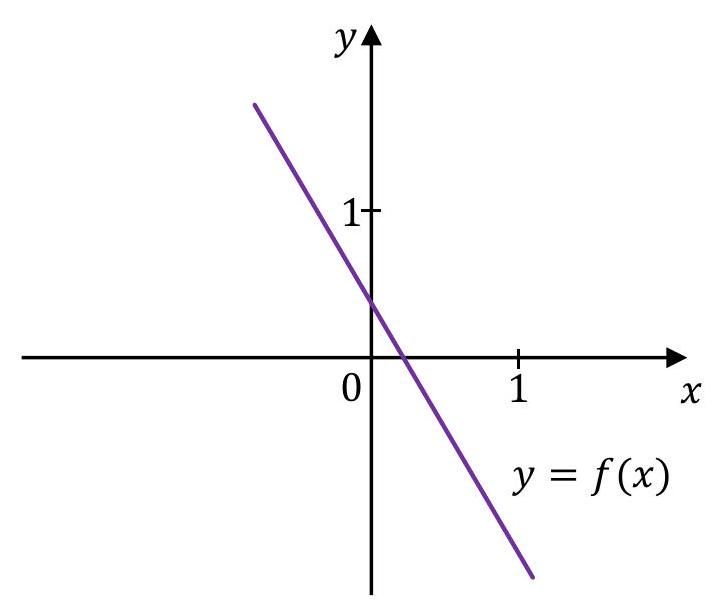
\includegraphics[max width=\textwidth, center]{2024_11_21_51cb67544fb9b029f01cg-13}

Dokończ zdanie. Wybierz właściwą odpowiedź spośród podanych.\\
Liczba \(a\) oraz liczba \(b\) we wzorze funkcji \(f\) spełniają warunki:\\
A. \(a>0\) i \(b>0\).\\
B. \(a>0\) i \(b<0\).\\
C. \(a<0\) i \(b>0\).\\
D. \(a<0\) i \(b<0\).\\

\includegraphics[max width=\textwidth, center]{2024_11_21_51cb67544fb9b029f01cg-13(1)}

Zadanie 14. (0-1) 마미\\
Jednym z miejsc zerowych funkcji kwadratowej \(f\) jest liczba (-5). Pierwsza współrzędna wierzchołka paraboli, będącej wykresem funkcji \(f\), jest równa 3.

Dokończ zdanie. Wybierz właściwą odpowiedź spośród podanych.

Drugim miejscem zerowym funkcji \(f\) jest liczba\\
A. 11\\
B. 1\\
C. \((-1)\)\\
D. \((-13)\)\\

\includegraphics[max width=\textwidth, center]{2024_11_21_51cb67544fb9b029f01cg-14}

Zadanie 15. (0-1) 두미이\\
Ciąg \(\left(a_{n}\right)\) jest określony wzorem \(a_{n}=2^{n} \cdot(n+1)\) dla każdej liczby naturalnej \(n \geq 1\).\\
Dokończ zdanie. Wybierz właściwą odpowiedź spośród podanych.\\
Wyraz \(a_{4}\) jest równy\\
A. 64\\
B. 40\\
C. 48\\
D. 80

\begin{center}
\begin{tabular}{|c|c|c|c|c|c|c|c|c|c|c|c|c|c|c|c|c|c|c|c|c|c|c|c|}
\hline
\multicolumn{4}{|l|}{Brudnopis} &  &  &  &  &  &  &  &  &  &  &  &  &  &  &  &  &  &  &  &  \\
\hline
 &  &  &  &  &  &  &  &  &  &  &  &  &  &  &  &  &  &  &  &  &  &  &  \\
\hline
 &  &  &  &  &  &  &  &  &  &  &  &  &  &  &  &  &  &  &  &  &  &  &  \\
\hline
 &  &  &  &  &  &  &  &  &  &  &  &  &  &  &  &  &  &  &  &  &  &  &  \\
\hline
 &  &  &  &  &  &  &  &  &  &  &  &  &  &  &  &  &  &  &  &  &  &  &  \\
\hline
 &  &  &  &  &  &  &  &  &  &  &  &  &  &  &  &  &  &  &  &  &  &  &  \\
\hline
 &  &  &  &  &  &  &  &  &  &  &  &  &  &  &  &  &  &  &  &  &  &  &  \\
\hline
 &  &  &  &  &  &  &  &  &  &  &  &  &  &  &  &  &  &  &  &  &  &  &  \\
\hline
 &  &  &  &  &  &  &  &  &  &  &  &  &  &  &  &  &  &  &  &  &  &  &  \\
\hline
 &  &  &  &  &  &  &  &  &  &  &  &  &  &  &  &  &  &  &  &  &  &  &  \\
\hline
 &  &  &  &  &  &  &  &  &  &  &  &  &  &  &  &  &  &  &  &  &  &  &  \\
\hline
 &  &  &  &  &  &  &  &  &  &  &  &  &  &  &  &  &  &  &  &  &  &  &  \\
\hline
 &  &  &  &  &  &  &  &  &  &  &  &  &  &  &  &  &  &  &  &  &  &  &  \\
\hline
\end{tabular}
\end{center}

\section*{Zadanie 16. (0-1) .}
Trzywyrazowy ciąg (27, 9, \(a-1\) ) jest geometryczny.\\
Dokończ zdanie. Wybierz właściwą odpowiedź spośród podanych.\\
Liczba a jest równa\\
A. 3\\
B. 0\\
C. 4\\
D. 2\\

\includegraphics[max width=\textwidth, center]{2024_11_21_51cb67544fb9b029f01cg-15}

Zadanie 17. (0-2)\\
Pan Stanisław spłacił pożyczkę w wysokości 8910 zł w osiemnastu ratach. Każda kolejna rata była mniejsza od poprzedniej o 30 zł.

Oblicz kwotę pierwszej raty. Zapisz obliczenia.\\

\includegraphics[max width=\textwidth, center]{2024_11_21_51cb67544fb9b029f01cg-16}

Zadanie 18. (0-1)\\
W kartezjańskim układzie współrzędnych \((x, y)\) zaznaczono kąt \(\alpha\) o wierzchołku w punkcie \(O=(0,0)\). Jedno z ramion tego kąta pokrywa się z dodatnią półosią \(O x\), a drugie przechodzi przez punkt \(P=(-3,1)\) (zobacz rysunek).\\
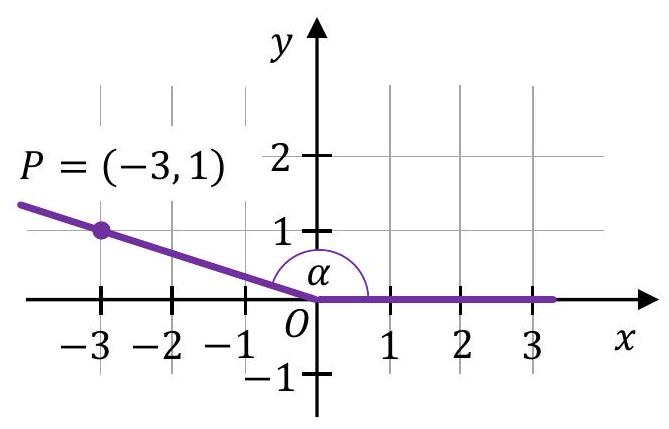
\includegraphics[max width=\textwidth, center]{2024_11_21_51cb67544fb9b029f01cg-17(2)}

Dokończ zdanie. Wybierz właściwą odpowiedź spośród podanych.\\
Tangens kąta \(\alpha\) jest równy\\
A. \(\frac{1}{\sqrt{10}}\)\\
B. \(\left(-\frac{3}{\sqrt{10}}\right)\)\\
C. \(\left(-\frac{3}{1}\right)\)\\
D. \(\left(-\frac{1}{3}\right)\)

\begin{center}
\begin{tabular}{|c|c|c|c|c|c|c|c|c|c|c|c|c|c|c|c|c|c|c|c|c|c|c|c|c|c|c|c|c|c|c|}
\hline
\multicolumn{5}{|l|}{Brudnopis} &  &  &  &  &  &  &  &  &  &  &  &  &  &  &  &  &  &  &  &  &  &  &  &  &  &  \\
\hline
 &  &  &  &  &  &  &  &  &  &  &  &  &  &  &  &  &  &  &  &  &  &  &  &  &  &  &  &  &  &  \\
\hline
 &  &  &  &  &  &  &  &  &  &  &  &  &  &  &  &  &  &  &  &  &  &  &  &  &  &  &  &  &  &  \\
\hline
 &  &  &  &  &  &  &  &  &  &  &  &  &  &  &  &  &  &  &  &  &  &  &  &  &  &  &  &  &  &  \\
\hline
 &  &  &  &  &  &  &  &  &  &  &  &  &  &  &  &  &  &  &  &  &  &  &  &  &  &  &  &  &  &  \\
\hline
 &  &  &  &  &  &  &  &  &  &  &  &  &  &  &  &  &  &  &  &  &  &  &  &  &  &  &  &  &  &  \\
\hline
 &  &  &  &  &  &  &  &  &  &  &  &  &  &  &  &  &  &  &  &  &  &  &  &  &  &  &  &  &  & 
\includegraphics[max width=\textwidth]{2024_11_21_51cb67544fb9b029f01cg-17}
 \\
\hline
\end{tabular}
\end{center}

\section*{Zadanie 19. (0-1)}
Dokończ zdanie. Wybierz właściwą odpowiedź spośród podanych.\\
Dla każdego kąta ostrego \(\alpha\) wyrażenie \(\sin ^{4} \alpha+\sin ^{2} \alpha \cdot \cos ^{2} \alpha\) jest równe\\
A. \(\sin ^{2} \alpha\)\\
B. \(\sin ^{6} \alpha \cdot \cos ^{2} \alpha\)\\
C. \(\sin ^{4} \alpha+1\)\\
D. \(\sin ^{2} \alpha \cdot(\sin \alpha+\cos \alpha) \cdot(\sin \alpha-\cos \alpha)\)\\

\includegraphics[max width=\textwidth, center]{2024_11_21_51cb67544fb9b029f01cg-17(1)}

Zadanie 20. (0-1) 무미이\\
W rombie o boku długości \(6 \sqrt{2}\) kąt rozwarty ma miarę \(150^{\circ}\).\\
Dokończ zdanie. Wybierz właściwą odpowiedź spośród podanych.\\
Iloczyn długości przekątnych tego rombu jest równy\\
A. 24\\
B. 72\\
C. 36\\
D. \(36 \sqrt{2}\)\\

\includegraphics[max width=\textwidth, center]{2024_11_21_51cb67544fb9b029f01cg-18(1)}

Zadanie 21. (0-1) 무민\\
Punkty \(A, B, C\) leżą na okręgu o środku w punkcie \(O\). Kąt \(A C O\) ma miarę \(70^{\circ}\) (zobacz rysunek).

\section*{Dokończ zdanie.}
Wybierz właściwą odpowiedź spośród podanych.\\
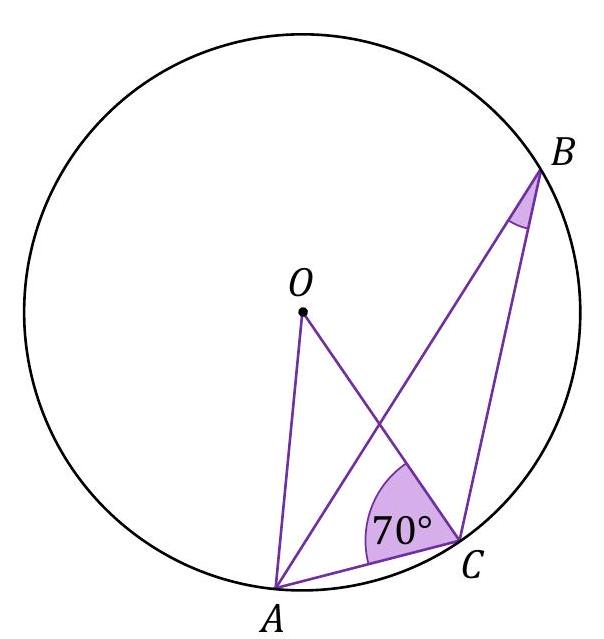
\includegraphics[max width=\textwidth, center]{2024_11_21_51cb67544fb9b029f01cg-18(2)}

Miara kąta ostrego \(A B C\) jest równa\\
A. \(10^{\circ}\)\\
B. \(20^{\circ}\)\\
C. \(35^{\circ}\)\\
D. \(40^{\circ}\)\\

\includegraphics[max width=\textwidth, center]{2024_11_21_51cb67544fb9b029f01cg-18}

Zadanie 22. (0-2)\\
Trójkąty prostokątne \(T_{1}\) i \(T_{2}\) są podobne. Przyprostokątne trójkąta \(T_{1}\) mają długości 5 i 12. Przeciwprostokątna trójkąta \(T_{2}\) ma długość 26.

Oblicz pole trójkąta \(T_{2}\). Zapisz obliczenia.\\

\includegraphics[max width=\textwidth, center]{2024_11_21_51cb67544fb9b029f01cg-19}

Zadanie 23. (0-1)\\
W kartezjańskim układzie współrzędnych \((x, y)\) dane są proste \(k\) oraz \(l\) o równaniach

\[
\begin{aligned}
& k: y=\frac{2}{3} x \\
& l: y=-\frac{3}{2} x+13
\end{aligned}
\]

Dokończ zdanie. Wybierz odpowiedź A albo B oraz odpowiedź 1., 2. albo 3.

Proste \(k\) oraz \(l\)

\begin{center}
\begin{tabular}{|l|l|l|l|l|}
\hline
A. & są prostopadłe &  & 1. & \((-6,-4)\) \\
\cline { 4 - 5 }
 & i przecinają się w punkcie \(P\) o współrzędnych & 2. & \((6,4)\) &  \\
\hline
B.\begin{tabular}{l}
nie są \\
prostopadłe \\
\end{tabular} &  & 3. & \((-6,4)\) &  \\
\hline
\end{tabular}
\end{center}

\begin{center}

\includegraphics[max width=\textwidth]{2024_11_21_51cb67544fb9b029f01cg-20}
\end{center}

Zadanie 24. (0-1) 마미\\
W kartezjańskim układzie współrzędnych \((x, y)\) dana jest prosta \(k\) o równaniu

\[
y=-\frac{1}{3} x+2
\]

\section*{Dokończ zdanie. Wybierz właściwą odpowiedź spośród podanych.}
Prosta o równaniu \(y=a x+b\) jest równoległa do prostej \(k\) i przechodzi przez punkt \(P=(3,5)\), gdy\\
A. \(a=3\) i \(b=4\).\\
B. \(a=-\frac{1}{3}\) i \(b=4\).\\
C. \(a=3\) i \(b=-4\).\\
D. \(a=-\frac{1}{3}\) i \(b=6\).

\begin{center}
\begin{tabular}{|c|c|c|c|c|c|c|c|c|c|c|c|c|c|c|c|c|c|c|c|c|c|c|c|c|c|c|c|c|c|c|}
\hline
\multicolumn{5}{|l|}{Brudnopis} &  &  &  &  &  &  &  &  &  &  &  &  &  &  &  &  &  &  &  &  &  &  &  &  &  &  \\
\hline
 &  &  &  &  &  &  &  &  &  &  &  &  &  &  &  &  &  &  &  &  &  &  &  &  &  &  &  &  &  &  \\
\hline
 &  &  &  &  &  &  &  &  &  &  &  &  &  &  &  &  &  &  &  &  &  &  &  &  &  &  &  &  &  &  \\
\hline
 &  &  &  &  &  &  &  &  &  &  &  &  &  &  &  &  &  &  &  &  &  &  &  &  &  &  &  &  &  &  \\
\hline
 &  &  &  &  &  &  &  &  &  &  &  &  &  &  &  &  &  &  &  &  &  &  &  &  &  &  &  &  &  & 
\includegraphics[max width=\textwidth]{2024_11_21_51cb67544fb9b029f01cg-21}
 \\
\hline
 &  &  &  &  &  &  &  &  &  &  &  &  &  &  &  &  &  &  &  &  &  &  &  &  &  &  &  &  &  & 
\includegraphics[max width=\textwidth]{2024_11_21_51cb67544fb9b029f01cg-21(3)}
 \\
\hline
 &  &  &  &  &  &  &  &  &  &  &  &  &  &  &  &  &  &  &  &  &  &  &  &  &  &  &  &  &  & 
\includegraphics[max width=\textwidth]{2024_11_21_51cb67544fb9b029f01cg-21(2)}
 \\
\hline
 &  &  &  &  &  &  &  &  &  &  &  &  &  &  &  &  &  &  &  &  &  &  &  &  &  &  &  &  &  & 
\includegraphics[max width=\textwidth]{2024_11_21_51cb67544fb9b029f01cg-21(7)}
 \\
\hline
 &  &  &  &  &  &  &  &  &  &  &  &  &  &  &  &  &  &  &  &  &  &  &  &  &  & 
\includegraphics[max width=\textwidth]{2024_11_21_51cb67544fb9b029f01cg-21(1)}
 & 
\includegraphics[max width=\textwidth]{2024_11_21_51cb67544fb9b029f01cg-21(4)}
 &  &  & 
\includegraphics[max width=\textwidth]{2024_11_21_51cb67544fb9b029f01cg-21(5)}
 \\
\hline
\end{tabular}
\end{center}

\section*{Zadanie 25. (0-1) 다}
Dany jest graniastosłup prawidłowy czworokątny, w którym krawędź podstawy ma długość 15. Przekątna graniastosłupa jest nachylona do płaszczyzny podstawy pod kątem \(\alpha\) takim, że \(\cos \alpha=\frac{\sqrt{2}}{3}\).

Dokończ zdanie. Wybierz właściwą odpowiedź spośród podanych.

Długość przekątnej tego graniastosłupa jest równa\\
A. \(15 \sqrt{2}\)\\
B. 45\\
C. \(5 \sqrt{2}\)\\
D. 10\\

\includegraphics[max width=\textwidth, center]{2024_11_21_51cb67544fb9b029f01cg-21(6)}

Zadanie 26. (0-4)\\
Dany jest ostrosłup prawidłowy czworokątny. Wysokość ściany bocznej tego ostrosłupa jest nachylona do płaszczyzny podstawy pod kątem \(30^{\circ}\) i ma długość równą 6 (zobacz rysunek).\\
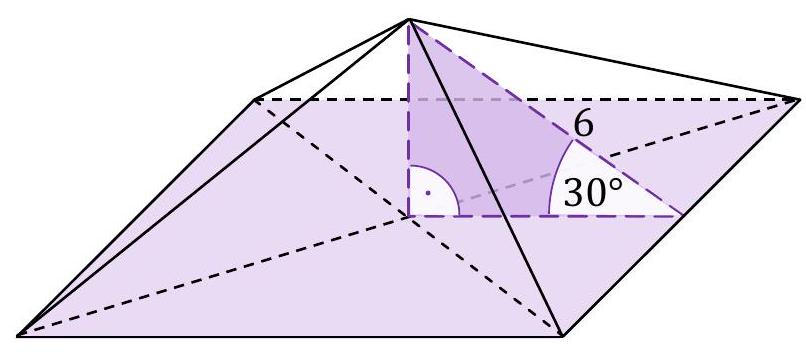
\includegraphics[max width=\textwidth, center]{2024_11_21_51cb67544fb9b029f01cg-22}

Oblicz objętość i pole powierzchni całkowitej tego ostrosłupa. Zapisz obliczenia.\\

\includegraphics[max width=\textwidth, center]{2024_11_21_51cb67544fb9b029f01cg-22(1)}\\

\includegraphics[max width=\textwidth, center]{2024_11_21_51cb67544fb9b029f01cg-23}

Zadanie 27. (0-1) 回回\\
W pewnym ostrosłupie prawidłowym stosunek liczby \(W\) wszystkich wierzchołków do liczby \(K\) wszystkich krawędzi jest równy \(\frac{W}{K}=\frac{3}{5}\).

Dokończ zdanie. Wybierz właściwą odpowiedź spośród podanych.

Podstawą tego ostrosłupa jest\\
A. kwadrat.\\
B. pięciokąt foremny.\\
C. sześciokąt foremny.\\
D. siedmiokąt foremny.\\

\includegraphics[max width=\textwidth, center]{2024_11_21_51cb67544fb9b029f01cg-24(1)}

\section*{\begin{center}

\includegraphics[max width=\textwidth]{2024_11_21_51cb67544fb9b029f01cg-24}
\end{center}}
Dokończ zdanie. Wybierz właściwą odpowiedź spośród podanych.

Wszystkich liczb naturalnych pięciocyfrowych, w których zapisie dziesiętnym występują tylko cyfry 0, 5, 7 (np. 57075,55 555), jest\\
A. \(5^{3}\)\\
B. \(2 \cdot 4^{3}\)\\
C. \(2 \cdot 3^{4}\)\\
D. \(3^{5}\)\\

\includegraphics[max width=\textwidth, center]{2024_11_21_51cb67544fb9b029f01cg-24(2)}

Zadanie 29. (0-2)\\
Na diagramie poniżej przedstawiono ceny pomidorów w szesnastu wybranych sklepach.\\
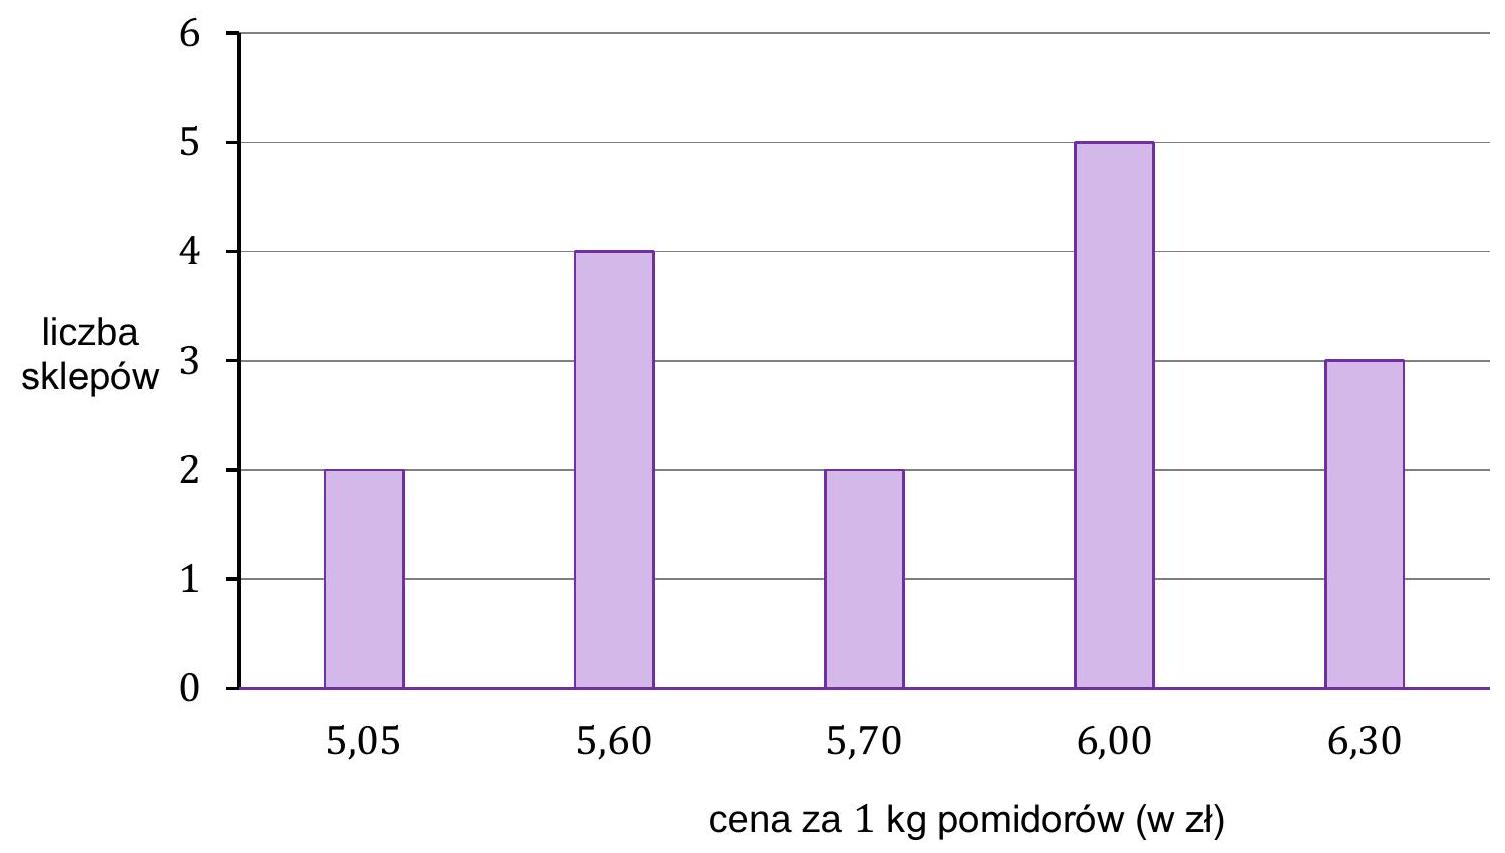
\includegraphics[max width=\textwidth, center]{2024_11_21_51cb67544fb9b029f01cg-25}

Uzupełnij tabelę. Wpisz w każdą pustą komórkę tabeli właściwą odpowiedź, wybraną spośród oznaczonych literami A-E.

\begin{center}
\begin{tabular}{|l|l|l|}
\hline
29.1. & \begin{tabular}{l}
Mediana ceny kilograma pomidorów w tych wybranych sklepach jest \\
równa \\
\end{tabular} &  \\
\hline
29.2. & \begin{tabular}{l}
Średnia cena kilograma pomidorów w tych wybranych sklepach jest \\
równa \\
\end{tabular} &  \\
\hline
\end{tabular}
\end{center}

A. \(5,80 \mathrm{zł}\)\\
B. 5,73 \(\mathrm{zł}\)\\
C. 5,85 \(\mathrm{zł}\)\\
D. 6,00 \(\mathrm{zł}\)\\
E. 5,70 \(\mathrm{zł}\)\\

\includegraphics[max width=\textwidth, center]{2024_11_21_51cb67544fb9b029f01cg-25(1)}

Zadanie 30. (0-2)\\
Ze zbioru ośmiu liczb \(\{2,3,4,5,6,7,8,9\}\) losujemy ze zwracaniem kolejno dwa razy po jednej liczbie.

Oblicz prawdopodobieństwo zdarzenia \(A\) polegającego na tym, że iloczyn wylosowanych liczb jest podzielny przez 15. Zapisz obliczenia.\\

\includegraphics[max width=\textwidth, center]{2024_11_21_51cb67544fb9b029f01cg-26}

\section*{Zadanie 31.}
Właściciel pewnej apteki przeanalizował dane dotyczące liczby obsługiwanych klientów z 30 kolejnych dni. Przyjmijmy, że liczbę \(L\) obsługiwanych klientów \(n\)-tego dnia opisuje funkcja

\[
L(n)=-n^{2}+22 n+279
\]

gdzie \(n\) jest liczbą naturalną spełniającą warunki \(n \geq 1\) i \(n \leq 30\).

Zadanie 31.1. (0-1) 다미\\
Oceń prawdziwość poniższych stwierdzeń. Wybierz P, jeśli stwierdzenie jest prawdziwe, albo F - jeśli jest fałszywe.

\begin{center}
\begin{tabular}{|l|c|c|}
\hline
\begin{tabular}{l}
Łączna liczba klientów obsłużonych w czasie wszystkich analizowanych dni \\
jest równa \(L(30)\). \\
\end{tabular} & P & F \\
\hline
W trzecim dniu analizowanego okresu obsłużono 336 klientów. & P & F \\
\hline
\end{tabular}
\end{center}

\begin{center}
\begin{tabular}{|c|c|c|c|c|c|c|c|c|c|c|c|c|c|c|c|c|c|c|c|c|c|}
\hline
\multicolumn{4}{|l|}{Brudnopis} &  &  &  &  &  &  &  &  &  &  &  & - &  &  & - &  &  &  \\
\hline
 &  &  &  &  &  &  &  &  &  &  &  &  &  &  &  &  &  &  &  &  &  \\
\hline
 &  &  &  &  &  &  &  &  &  &  &  &  &  &  &  &  &  &  &  &  &  \\
\hline
 &  &  &  &  &  &  &  &  &  &  &  &  &  &  &  &  &  &  &  &  &  \\
\hline
 &  &  &  &  &  &  &  &  &  &  &  &  &  &  &  &  &  &  &  &  &  \\
\hline
 &  &  &  &  &  &  &  &  &  &  &  &  &  &  &  &  &  &  &  &  &  \\
\hline
 &  &  &  &  &  &  &  &  &  &  &  &  &  &  &  &  &  &  &  &  &  \\
\hline
 &  &  &  &  &  &  &  &  &  &  &  &  &  &  &  &  &  &  &  &  &  \\
\hline
 &  &  &  &  &  &  &  &  &  &  &  &  &  &  &  &  &  &  &  &  &  \\
\hline
 &  &  &  &  &  &  &  &  &  &  &  &  &  &  &  &  &  &  &  &  &  \\
\hline
\end{tabular}
\end{center}

Zadanie 31.2. (0-2)\\
Którego dnia analizowanego okresu w aptece obsłużono największą liczbę klientów? Oblicz liczbę klientów obsłużonych tego dnia. Zapisz obliczenia.\\

\includegraphics[max width=\textwidth, center]{2024_11_21_51cb67544fb9b029f01cg-27}\\

\includegraphics[max width=\textwidth, center]{2024_11_21_51cb67544fb9b029f01cg-28}

BRUDNOPIS (nie podlega ocenie)\\

\includegraphics[max width=\textwidth, center]{2024_11_21_51cb67544fb9b029f01cg-29}\\
\includegraphics[max width=\textwidth, center]{2024_11_21_51cb67544fb9b029f01cg-30}\\
\includegraphics[max width=\textwidth, center]{2024_11_21_51cb67544fb9b029f01cg-31}

\section*{MATEMATYKA}
\section*{Poziom podstawowy}
Formuła 2023

\section*{MATEMATYKA}
\section*{Poziom podstawowy}
Formuła 2023

\section*{MATEMATYKA}
\section*{Poziom podstawowy}
Formuła 2023


\end{document}